
%----------------------------------------------------------------
%
%  File    :  komponenten.tex
%
%  Authors :  ???
% 
%  Created :  7 Sept 2019
% 
%  Changed :  7 Sept 2019
% 
%---------------------------------------------------------------


\section{Komponenten}
\label{sec:Komponenten}
	\subsection{Use Cases}
	\label{subsec:Use Cases}
	
	Aufgrund der Tatsache dass, sich das 4G LTE Mobilfunknetz über verschiedene Sektoren wie dem Öffentlichen Dienst, der Energieversorgung, dem Transportwesen, wie auch dem Bildungsbereich sowie auch dem Gesundheitswesen erstrecken soll, ergeben sich als Anforderungen vor allem eine hohe Abdeckung, sowie hohe Datenraten, welche für die Benutzer, also die Inselbewohner, verfügbar sein sollen \cite{Tch18}. 

Zusätzlich verfügt die zu betrachtende Insel über ein Seenotrettungssystem, präziser gesagt ein maritimes Rettungs-Koordinationszentrum, über welches mit Hilfe von Rettungsschiffen und Rettungsdrohnen in Seenot geratene Inselbewohner lokalisiert werden können \cite{eckermann2018tinylte}. Des Weiteren bewegen sich die Einwohner auf dem Staatsgebiet der Insel in autonom fahrenden Autos, weshalb auch hierfür entsprechende Anforderungen in Bezug auf die Komponenten für vehikulare Kommunikation bei der Planung eines Mobilfunknetzes berücksichtigt werden sollte. Da eine Infrastruktur von Grund auf erbaut wird, muss keine Rücksicht auf etwaige bestehende Legacy Architekturen genommen werden, in welche neue Komponenten zu integrieren sind. 
\subsection{State of the Art Marktanalyse}
\label{subsec:Marktanalyse}

Um die ansäßigen Inselbewohner zufrieden zustellen, sollten insbesondere Peak Data Raten, die Zellkapazitäten, der Zellradius, die Radio Access Modi, die Antennen Schemata, sowie das Mobility Speed Handover konkreter in Erwägung gezogen werden\cite{Dat14}.
Bei der Recherche zur Thematik haben sich folgende Kriterien als Unterscheidungsmerkmale herauskristallisiert, welche eine Entscheidungsfindung beeinflussen. Ob nun anhand dieser letztlich eine Entscheidung getroffen wird, ob nun ein Mobilfunknetz selbst errichtet (Make) oder die notwendigen Komponenten (Buy) hinzugekauft werden sollen, wird im Kapitel Make or Buy näher beleuchtet. Neben dem Spektrum, dem Durchsatz (Throughput), der Latenz (Latency), der Redundanz (Redundancy), der Interoperabilität beziehungsweise der Kompatibilität, ist auch die Möglichkeit der Skalierbarkeit, um etwaige Nachbarinseln mitzuversorgen, von signifikanter Bedeutung. Denn diese haben ihrerseits kooperativ ihre Hilfe zur Analyse der Problematik in Form der Nutzung eines Internet Cafes angeboten, um erste Recherchearbeit bezüglich des Aufbaus eines LTE Mobilfunknetzes zu liefern. Zusätzlich  als weitere nicht zu vernachlässigende Elemente stellen auch Kriterien wie das des Monitorings respektive des Control Managements, ebenso wie dem möglichen Coverage, als auch die Kapazität Faktoren dar, welche die finalen Entscheidungsprozesse maßgeblich beeinflussen. Zudem sollte abzuwägen sein, ob ein "Easy to use enerprise Dashboard" vorhanden ist. Des Weiteren wird wichtig zu prüfen, ob Lincesing an für sich eine Problematik darstellen könnte. Inwiefern auf der Südsee Insel nach internationalem Recht bzw. in welchen gesetzlichen Rahmenbedingungen die Verantwortlichen Projektleiter sich bewegen und dementsprechend danach handeln.
	\subsection{Anbieter am Markt}
	\label{subsec:Anbieter am Markt}
	Eine Vielzahl von Anbietern für die Errichtung eines Mobilfunknetzes bestimmen derzeit den globalen LTE Advanced Markt.\ Die dominierenden Unternehmen an diesem sind neben Ambra Solutions, Arris International,
	Athonet, Cisco, Comba, DruidSoftware, Ericsson, Future Technologies, General Dynamics und 
	Huawei. Neben diesen existieren aber auch weitere Anbieter wie beispielsweise Lemko, Luminate Wireless,
	Mavenir,
	NEC,
	Netnumber,
	Nokia,
	Pdvwireless,
	Quortus,
	Redline Communications,
	Samsung,
	Sierra Wireless,
	Star Solutions,
	Ursys,
	Verizon und 
	Zinwave \cite{Max19}.
	Abhängig von den Use Cases ergeben sich bei der Analyse und beim Design spezifizierte funktionale wie auch Nicht-funktionale Anforderungen. Durch die konkrete Betrachtung einer Einführung eines Mobilfunknetzes gilt es, sich mit auftretenden Fragestellungen wie  dem Angebot an qualifiziertem Fachpersonal, welches auf den LTE Advanced Standard geschult ist, auseinander zu setzen. Dieses kann dann sowohl in den Phasen der Analyse und des Designs als auch in denen der Implementierung sowie bei Wartung und beim Testen vor Inbetriebnahme gezielt eingesetzt werden. Ist entsprechendes Kapital vorhanden, eine Armada externer Berater einzufliegen, die schon einmal ähnliche Projekte realisiert haben, um mit Hilfe derer Erfahrungswerte von vergangenen Projekten in Bezug auf Planung, Koordination und Aufwandsabschätzungen zu nutzen und somit Fehleinschätzungen zu minimieren im ideal Fall zu vermeiden. Sind generell Fachkräfte mit domain spezifischem Know-How verfügbar oder ist es sinnvoll Schulungszentren aufzubauen, um langfristig Abhängigkeiten von Schulungsdienstleistern zu verringern.
%	\subsection{HSS, EPC, PCRF}
%	\label{subsec:Antennen HSS, EPC, PCRF}
%		\subsection{Preise der Komponenten}
%	\label{subsec:Preise der Komponenten}
	\subsection{Antennen Konfigurationen}
	\label{subsec:Antennen Konfigurationen}
Bevor man die Komponenten, welche von unterschiedlichen Marktteilnehmern angeboten werden vergleicht, ist es durchaus sinnvoll ein Bild über die Empfangsbedingungen in dem Inselstaat machen. Abhängig von physikalischen Einflussfaktoren in Form von Waldgebieten, Gebäudekomplexen oder topologischen Strukturen wie Gebirge sie darstellen, können ebensolche signifikant die Signalübertragung bestimmen. Denn schließlich sind Absorption, Beugung oder auch Reflexion mit die Hauptgründe für Störungen bei der Ausbreitung elektromagnetischer Wellen. Um nun einen optimalen Empfang zu gewähren kann eine Kombination aus Antennentypen angedacht werden, da jede einzelne Bauart ihre Vor- und Nachteile aufweist. So ist zu unterscheiden zwischen Mono- und Breitband Antennen. Mono-Antennen sind hierbei der Klasse der Richtantennen und Breitbandantennen der Klasse der Rundstrahler zuzuordnen. \cite{Sch19}
\begin{figure*}[ht]
	\centering
	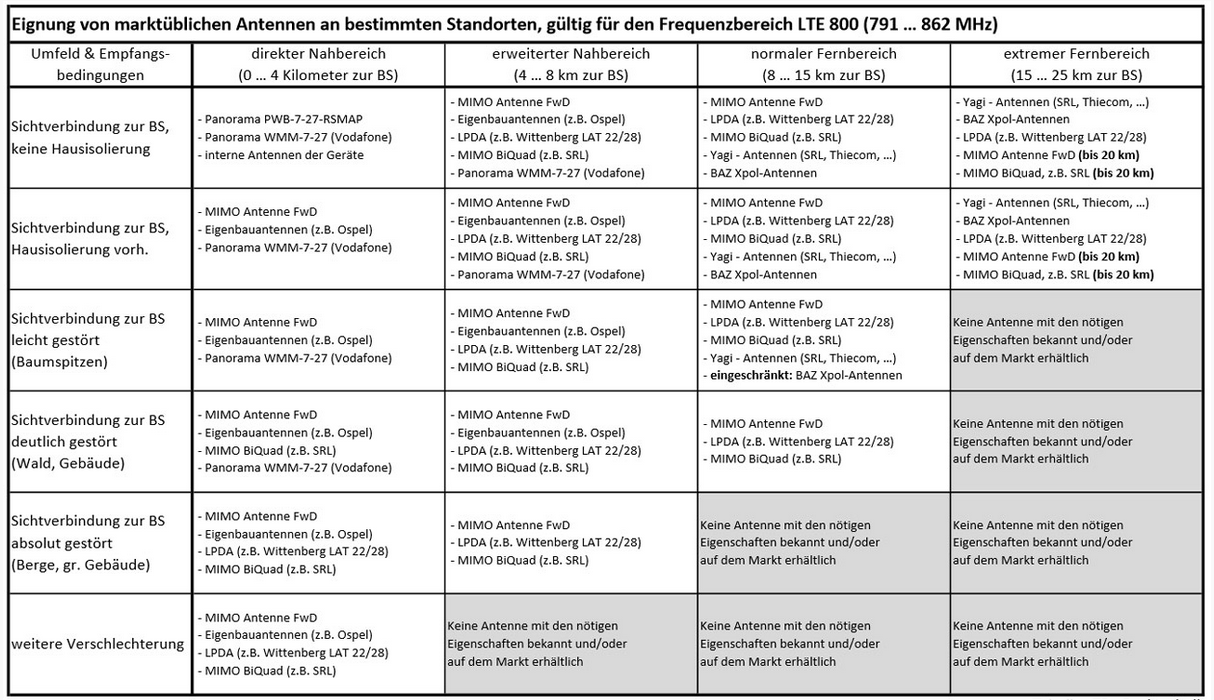
\includegraphics[width=1\linewidth]{images/tabellemcnantennen}
	\caption{Antennenüberblick  \protect\cite{Sch19}}
	\label{fig:tabellemcnantennen}
\end{figure*}

%\newpage
 %\flushbottom 
%\nextpage
\raggedbottom 
